\subsection{Drivetrain}
\subsubsection{Rescue Robot Drivetrain}
The drivetrain is the system in a motor vehicle which connects the transmission to the drive axle. In regard to a rescue robot the drivetrain is made up of the motors (and their controllers), the drive axles, the cams (drive wheels), the tracks and all parts in-between. The drivetrain of the rescue robot is a crucial component as without it the robot would have no mobility.\par
The balance between power and speed must also be well thought out. Too little power would mean the robot would be unable to traverse the uneven surfaces of disaster zones and not enough speed would result in a prolonged time to survey and manoeuvre within a disaster zone. The drivetrain of rescue robots are usually tracked rather than wheeled in order to navigate unpredictable terrain. This makes rescue robot control unique.

%Rational of Previous Design%
\subsubsection{Rational of Previous Design (2014/15)}
The drivetrain of Orion (2014/15) was modelled by breaking the design down into three sections; steering, suspension and tracks. These three separate sections ultimately dictated the requirements for their drivetrain and will therefore be used as a basis to review the design of last year’s drivetrain.\par

The steering was designed with the intention of using a skid method which uses two separate motors (one per track) allowing each track to be controlled independently, this is known as dual drive. The skid steering method is one of the more efficient ways of controlling a tracked vehicle as it allows continuous movement whilst turning. The selection behind the steering was sound and the dual drive, skid steering will be used in Cyclone’s (2015/16) design.\par

The tracks were chosen using consultation from experts at Transdev (the track supplier) and analysis of previous designs of WMR robots. Specialist rubber tracks were selected for Orion due to the high durability and traction, and multi-terrain capability. The track layout was also designed with the intention of making Orion invertible (able to drive when flipped over).\par

The motors for Orion were selected using values of worst case acceleration and power required. These conditions were accelerating at 0.3$ms^-2$ up an incline of 38\textordmasculine (the incline of a standard step) with an estimated robot weight of 25kg. These values gave a required torque of 4.95Nm per motor. This resulted in the EC-4pole 22 \o22 mm, brushless, 90 Watt (specification found in Appendix) motor being selected. A gearhead was required to work alongside this motor to reach the torque required. This gearhead was selected to meet the torque requirements of the Orion project (4.95Nm) and can be seen in the Appendix. The location of Orion’s motors were selected with the premise of saving space, allowing more room to locate other components, in particular the sensor array, they were therefore positioned towards the back of the robot (figure \ref{fig:Orionmotorlayout}).\par

%Insert figure XX1 'Orion (2015/16) internal motor layout' (center aligned)%
\begin{figure}[h]
\centering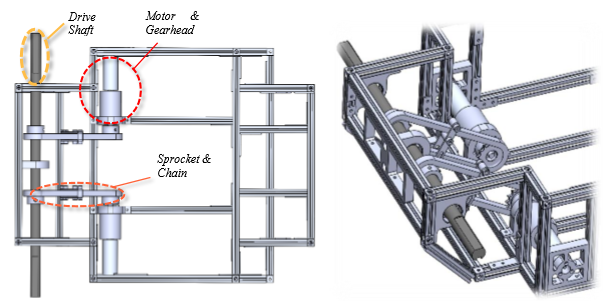
\includegraphics[width=0.6\linewidth]{Images/DT_Fig_1.png}
\caption{Orion (2015/16) internal motor layout}
\label{fig:Orionmotorlayout}
\end{figure}

The RPM required of the motor was governed by the competition specifications which were to accelerate at 0.3$ms^-2$ and have standard operation at 1$ms^-1$. Using the speed constant of Orion’s motors ($907 rpmV^-1$) and the battery’s maximum (24V) and minimum (18V) voltage the speed operating window can be obtained, this is 81.76-109.02rpm and 0.43-0.57$ms^-1$. This was below the  standard operating condition.\par

\subsubsection{Critical Analysis of Previous Design (2014/15)}
The design and reasoning behind the steering system was sound and was the only real option for the type of dual tracked robot that is being built in this project. Using separate motors to control each track will give enhanced mobility and will allow for a more fluid movement than if one motor was used. This design is also the simplest method of control as it does not involve a clutch or gearing system like the alternatives. Thus, the dual drive method of controlling the robot will be carried forward into Cyclone (2015/16).\par

The material selection for the tracks was sensible and the use of the expertise of the Transdev team will be used to select the tracks for Cyclone (2015/16). The specialist rubber design gives the tracks the flexibility they need not only to travel around the drive wheels and guide wheels but also to react to the uneven terrain of a disaster zone. This in conjunction with our new suspension design will allow for improved traction when traversing this uneven terrain. The track design of Orion was also created with the intention of allowing it to drive when upside down, this meant that it encompasses the area around the body. This invertible design would be void if their suggestion of improvement by the addition of a robot arm was carried out, this would obviously not allow the robot to travel both the right way up and upside down. After consideration of the profile of Orion’s track design it was made clear that the tractive length was too short to allow the robot to climb stairs. The distance between the two points of consecutive steps is 308.8mm (figure \ref{fig:Orionstairs} and \ref{fig:Cyclonestairs}) and the tractive length of Orion was only 244.60mm, whereas Cyclone’s new extended parallelogram track profile allows it to easily climb a standard step (figure \ref{fig:Cyclonestairs}).\par

%These figure are on the same level%
%Insert figure XX2 'Orion struggling to climb standard stairs',(left aligned)%
%Insert figure XX3'Cyclone easily climbing standard stairs', (right aligned)%
\begin{figure}[h]
\centering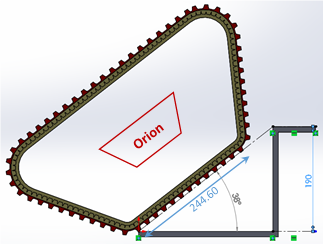
\includegraphics[width=0.5\linewidth]{Images/DT_Fig_2.png}
\caption{Orion struggling to climb standard stairs}
\label{fig:Orionstairs}
\end{figure}

\begin{figure}[h]
\centering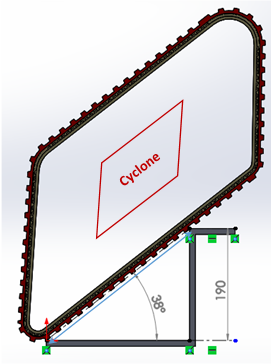
\includegraphics[width=0.4\linewidth]{Images/DT_Fig_3.png}
\caption{Cyclone easily climbing standard stairs}
\label{fig:Cyclonestairs}
\end{figure}

As mentioned in the previous section the motor and gearhead combination were selected using the worst case scenario of accelerating a 25kg Orion at 0.3$ms^-2$ up an incline of 38\textordmasculine. This calculation gave a required torque of 4.95Nm per motor. This torque was found by assuming 80\% efficiency of the motor and gearhead combination, when in fact the selected motor was 88\% efficient and the gearhead was 77\% efficient giving a total efficiency of 67.76\%. Using the actual efficiency, the worst case scenario torque required for Orion would be 5.79Nm. This highlights the point that the efficiency should have been thoroughly researched and a sensible estimate made from the Maxon Motor data available. The stall torque was also taken into consideration and so a motor with a minimum stall torque of 25Nm was suggested (about five timed times the worst case torque). With this in mind a motor with a stall torque of 0.588Nm and a gearhead with a 123:1 reduction were selected giving an overall torque output of 72.32Nm (if 100\% efficiency and maximum running is assumed). Orion has a system with 67.76\% efficiency and so therefore, using the nominal current and torque constant for Orion’s motors, one can see that this combination is not suited for accelerating the 25kg Orion up a 38\textordmasculine slope as it only provides 3.45Nm rather than the 5.79Nm required. Further analysis using a simple force diagram (figure \ref{fig:slopeforce}) shows that a total force of 150.99N is required to hold a weight of 25kg still on a 38\textordmasculine slope. This equates to 75.5kg and 3.77Nm per motor, which is greater than the torque that Orion’s motors provide. The motor and gearhead selected for Orion will render the robot useless whenever it comes to any obstacle.\par

%Insert figure XX4 'Simple force diagram for Orion on a 38deg slope' (center aligned)%
\begin{figure}[h]
\centering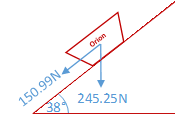
\includegraphics[width=0.4\linewidth]{Images/DT_Fig_4.png}
\caption{Simple force diagram for Orion on a 38\textordmasculine slope}
\label{fig:slopeforce}
\end{figure}

The speed of the motors was also lacking, only giving a maximum speed of 0.57$ms^-1$. This speed would not be maintained as this was calculated assuming the battery had maximum charge. Realistically the speed would be more around the lower value of 0.43$ms^-1$.\par

There is always a trade-off between speed and torque but it is hard to see here which factor was favoufavouredred  in the design of Orion’s drivetrain, as neither the speed nor the torque are sufficient for the successful operation of the robot. For this reason a new motor and gearhead selection will be made for Cyclone.\par

%Review of Alternative Drivetrain Designs%
\subsubsection{Review of alternative Drivetrain Design}

There are a number of different methods that can be used to propel a vehicle, this section will explore a number of options and justify the option chosen.\par

\paragraph*{Propulsion}

Firstly, the robot needs a way of converting power to forward momentum. Choosing the best system depends on several factors including the traction, steering, suspension and the ground pressure. Three methods of delivering movement were explored; wheels, tracks and legs.\par

\subparagraph*{Wheels}
%insert reference for this section http://www.intorobotics.com/wheels-vs-continuous-tracks-advantages-disadvantages/%
This is the most common method of movement in ground vehicles and so the possibility was explored for Cyclone.\par

Wheels provide a simple platform for movement as there are limited moving parts involved, namely only the wheel and drive axle will be turning. This means that there are fewer components that could get damaged. If there was ever any damage however, the simplicity of design would mean the repair would be quick, easy and cheap. This simplicity would also mean constructing a wheeled robot, including the suspension element, would be easier and cheaper than a more complicated design such as a tracked variant.\par

The wheeled design offers a high degree of manoeuvrability and allows the robot to travel at high speeds compared with tracks and legs, this due to the wheels needing a lower torque to start and continue moving. This high degree of manoeuvrability also makes the wheeled robot easy to control. Figure \ref{fig:wheelturn} shows the method of turning for a wheeled vehicle, the robot can turn on the spot by driving the left wheels forward and the right wheels backwards. The steering of a wheeled robot could also be carried out using the same method as a car (bell-crank and rack-and-pinion steering linkage).\par

%Insert figure XX5 'Turning Method of a wheeled robot' (center aligned)%
\begin{figure}[h]
\centering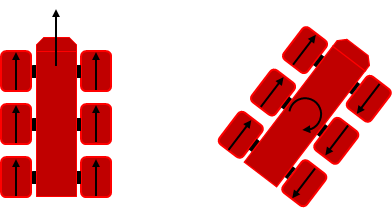
\includegraphics[width=0.6\linewidth]{Images/DT_Fig_5.png}
\caption{Turning Method of a wheeled robot}
\label{fig:wheelturn}
\end{figure}

Because wheels have been around for such a long time they have seen a number of advancements in their design and so there are a number of variants of the wheel, shown below (Figure \ref{fig:Wheeltype}).\par

%Insert figure XX6 'Different Wheel types for a Robot' (center aligned)%
\begin{figure}[h]
\centering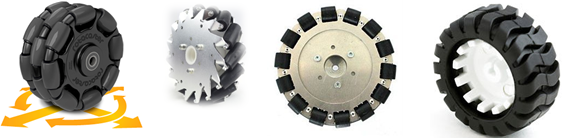
\includegraphics[width=0.6\linewidth]{Images/DT_Fig_6.png}
\caption{Different Wheel types for a Robot}
\label{fig:Wheeltype}
\end{figure}
%References for figure (left to right: Omni https://en.wikipedia.org/wiki/Omni_wheel%
%mecanum http://robu.in/shop/152mm-aluminium-mecanum-wheel-right/%
%omnidirectional http://www.robotshop.com/en/152mm-omnidirectional-wheel.html%
%standard https://www.sparkfun.com/products/8899%

Although they have a large variety of designs available and their simplicity makes them cheap and easy to build wheels do have their disadvantages. The first and main disadvantage is that wheels must be at least twice the height of an obstacle in order to overcome it, so in the case of climbing a standard staircase the wheel must be 380mm high. The second major disadvantage is the small contact area with the ground resulting in reduced traction. This small contact area also means the weight is concentrated at specific points making wheeled vehicles unsuitable for soft terrain.\par

\subparagraph*{Tracks}
%insert reference for this section http://www.intorobotics.com/wheels-vs-continuous-tracks-advantages-disadvantages/%

Tracks are an alternative to the wheeled design although they offer a more complex system. Unlike a wheeled design tracks have a low ground impact as the weight is distributed along the track length in contact with the ground. This is ideal for a disaster zone where survivors may be trapped under rubble. The larger footprint of the track offers increased traction and therefore a higher performance efficiency compared to wheels. The increased traction coupled with the flexibility of the continuous tracks also allows for the traversing of rough terrain where a wheeled design would get stuck due to its single contact points.\par

The steering system is as simple as the wheeled design (figure \ref{fig:trackturn}) allowing for on the spot turning and good manoeuvrability.\par

%Insert figure XX7 'Turning Method of a tracked robot' (center aligned)%
\begin{figure}[h]
\centering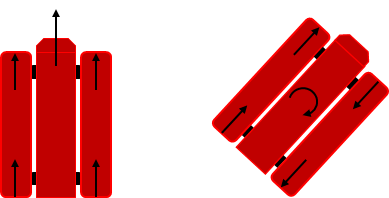
\includegraphics[width=0.6\linewidth]{Images/DT_Fig_7.png}
\caption{Turning Method of a tracked robot}
\label{fig:trackturn}
\end{figure}

Although the tracked design is better suited to the rough terrain of a disaster zone it does offer less precise movement and due to the increased traction more power is required whilst turning. The overall design tends to be bulky and heavier and given the more complex nature the build and repair tend to be more costly than alternatives.\par

\subparagraph*{Legs}
%insert reference for this section https://www.quora.com/Is-there-any-benefit-to-legged-robots-over-wheeled-ones%

Legs are becoming more and more common in robot designs and so they were considered for Cyclone.\par

Legs are the most agile of the three options and rather than being able to perform at high speeds they enable the robot to react quickly to any outside forces or changes in environment, allowing a change in pose or principal orientation. This reactiveness allows for an extremely stable platform for the robot when walking over ice, mud, rocks etc. A legged robot also has the advantage of the environment being designed specifically for legged/limbed locomotion (humans). Limbs (of a robot) also allow a greater ‘solution space’ giving more options when traversing uneven surfaces and obstacles (figure \ref{fig:solutionspace}). The limbs of the robot could also be utilised to climb vertical surfaces allowing the exploration of areas tracked or wheeled robots could not reach (figure \ref{fig:legclimb}).\par

%Insert figure XX8 'Solution Space of a legged robot' (center aligned)%
\begin{figure}[h]
\centering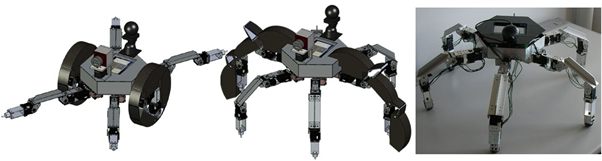
\includegraphics[width=0.6\linewidth]{Images/DT_Fig_8.png}
\caption{Solution Space of a legged robot}
\label{fig:solutionspace}
\end{figure}
%Insert figure XX9 'Legged Robot Climbing a vertical surface' (center aligned)%
\begin{figure}[h]
\centering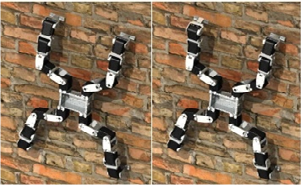
\includegraphics[width=0.6\linewidth]{Images/DT_Fig_9.png}
\caption{Legged Robot Climbing a vertical surface}
\label{fig:legclimb}
\end{figure}

As well as the physical advantages, a limbed robot would be a more sensible choice in terms of set-up and cost for a disaster extraction, because no local infrastructure would have to be set up, like paths and open passages.\par

The limb design is still in research and so is currently expensive and extremely time consuming to get right on a project dealing with such unpredictable environments. This is the main downfall of this type of design.\par

\subparagraph*{Choice}

Considering the three options above the best choice for Cyclone would be a tracked drivetrain. The main reason for this is because of its more rugged nature and greater ability to traverse the uneven terrain it will encounter in a disaster zone.\par

\paragraph*{Manoeuvrability}

The method of steering is the next factor to consider now that tracks have been selected for the drivetrain. There are a number of way to steer a two track vehicle and this section will explore five options and ultimately decide the best of these.\par
%Not all of these need to be in the text, a couple can go in the appendix%

\subparagraph*{Dual Drive}

This is the simplest way to steer a dual tracked vehicle and requires a separate power source (motor) for each track.\par

In order to steer this system one motor is supplied with more power than the other, this results in one track travelling faster (and so further) than the other causing a turning moment. This design also allows the vehicle to perform a neutral turn (turn on the spot) by driving one motor forward and the other in reverse. This will be useful when navigating the tight environment of a disaster zone. The simplicity of the design make the steering intuitive and so the vehicle is easy to operate often using one throttle ‘stick’ per motor, allowing any unskilled personnel to pick up a controller and operate the vehicle.\par

This design does come with some disadvantages. Two power sources means double the chance of something going wrong and so reliability will be lower than a system with one motor. If one motor was to fail the vehicle would be immobilised and capable of only spinning in circles, rendering it useless. Another issue with two motors is there will be double the weight, and with the motors tending to be near the drive wheels (at the back) this presents an issue with the centre of gravity. The final issue would be the ease of steering. It may be difficult to supply the same amount of power through each motor and still maintain a straight line. If the same power is supplied to each motor to travel in a straight line, there would still be the issue of each track not experience the same amount of drag causing the tracks to turn at slightly different speeds. This tends not to be an issue at lower speeds.\par

%Insert figure X10 'Dual Drive Layout' (center aligned)%
\begin{figure}[h]
\centering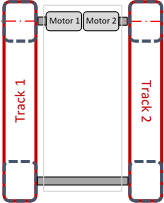
\includegraphics[width=0.4\linewidth]{Images/DT_Fig_10.png}
\caption{Dual Drive Layout}
\label{fig:dualdrive}
\end{figure}

\subparagraph*{Clutch Brake}

This method only requires one motor which drives both tracks directly. This technique involves disengaging one track from the motor via a clutch mechanism (figure \ref{fig:clutchbrake}) in order to slow the disengaged track until it comes to a stop. The other track is still engaged and traveling at the speed of the motor, so causing a turning effect. The disengaged track can also use a brake to bring it to an immediate stop allowing a tighter turning radius. This is another easy method of controlling a tracked vehicle it is however not very efficient. The constant stopping and accelerating of the tracks also makes manoeuvring slow and inefficient, because by slowing and braking one track in order to turn energy is wasted from the motor. This method also does not allow on the spot turning which would cause problems in the tight areas within a disaster zone.\par

%Insert figure X11 'Clutch Brake Layout' (center aligned)%
\begin{figure}[h]
\centering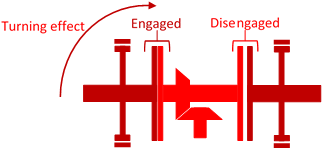
\includegraphics[width=0.6\linewidth]{Images/DT_Fig_11.png}
\caption{Clutch Brake Layout}
\label{fig:clutchbrake}
\end{figure}

\subparagraph*{Gearing Steering}

In a gearing steering system a single motor is used to power both sets of tracks through separate transmissions. The tracked vehicle is steered by selecting different gears for each of the tracks. In figure \ref{fig:gearSteer} the $1^{st}$ gear is engaged on the left side and the $2^{nd}$ gear is engaged on the right side, this will result in the left track travelling at a lower speed than the right and so giving a left hand turning effect. This method allows for a smooth and efficient method of steering the vehicle and allows a large combination of gearing ratios to be used for a large number of turning radii. Another advantage of this method is that each transmission can incorporate a reverse gear and so a neutral turn is possible. However, this method is complex in nature and correct implementation can be time consuming and costly.\par

%Insert figure X12 'Gearing Steering Layout' (center aligned)%
\begin{figure}[h]
\centering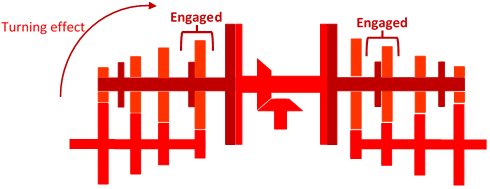
\includegraphics[width=0.6\linewidth]{Images/DT_Fig_12.png}
\caption{Gearing Steering Layout}
\label{fig:gearSteer}
\end{figure}

\subparagraph*{Braked Differential}

This is a simplified version of the clutch-brake drive shown above. The two axles are driven through a differential and so eliminating the clutches. When one axle is slowed or stopped the differential acts to transfer all the motion to the remaining ‘free’ axel and so resulting in a turning effect. This method is however less efficient than the clutch-brake system, given the brake dissipates the energy of the track and the motor. The braked differential method is also harder to control and straight line travel may become a problem as the system can become unpredictable. However, Its simplicity makes up for these faults.\par

%Insert figure X13 'Braked Differential Layout' (center aligned)%
\begin{figure}[h]
\centering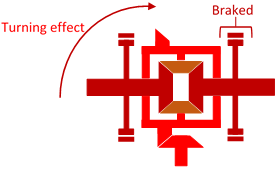
\includegraphics[width=0.6\linewidth]{Images/DT_Fig_13.png}
\caption{Braked Differential Layout}
\label{fig:brakeddiff}
\end{figure}

\subparagraph*{Double Differential}

This is a more refined version of the standard braked differential system. This method adds a second transmission between the steering input of the transmission and the motor. This allows the differential gears to be run at several different speeds resulting in a large combination of track speeds. This will allow for a great number of turning radii making this system extremely well suited for fast steering vehicles. This system is used for all modern fast track-layer steering transmissions due to its efficiency, turning radii possibilities (including a neutral turn) and its stability (it won’t self-steer).\par

%Insert figure X14 'Double Differential Layout' (center aligned)%
\begin{figure}[h]
\centering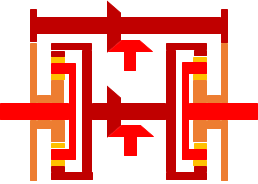
\includegraphics[width=0.4\linewidth]{Images/DT_Fig_14.png}
\caption{Double Differential Layout}
\label{fig:doublediff}
\end{figure}

\subparagraph*{Choice}

Due to the simplicity of its design and the ease of use the dual drive option was chosen to power Cyclone.\par

\subsubsection{Design of Cyclone's Drivetrain}

Cyclone’s drivetrain was created from scratch given the new modular design implemented for this build and the drawbacks of the previous year’s design. Within the modular build the rear module is solely dedicated to the drivetrain. As mentioned above tracks were chosen along with a dual drive system for Cyclone allowing it to easily traverse the unpredictable terrain found within a disaster zone.\par

The motors for Cyclone were considered against the amended worst case requirements, this is accelerating 30kg at 0.3$ms^-2$ up an incline of 38\textordmasculine. Cyclone is predicted to have a slightly heavier weight of 30kg as its design is intended to be added to in future projects and so taking into account a heavier weight will allow the same drive system to be used in the future.\par

According to the simple force diagram (figure \ref{fig:simpleforcecyclone}) Cyclone will require a force of 181.19N to keep it stationary on an incline of 38\textordmasculine, that is 90.59N per motor.\par

%Insert figure X15 'Simple force diagram for Cyclone on a 38deg incline' (cneter aligned)%
\begin{figure}[h]
\centering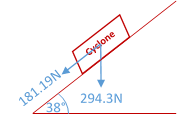
\includegraphics[width=0.4\linewidth]{Images/DT_Fig_15.png}
\caption{Simple force diagram for Cyclone on a 38\textordmasculine incline}
\label{fig:simpleforcecyclone}
\end{figure}

The minimum amount of torque required in this worst case scenario can be found by simplifying figure \ref{fig:simpleforcecyclone} to a wheel travelling up a slope (figure \ref{fig:simpleforcewheel}).

%Insert figure X16 'Simple force diagram for a wheel on a 38deg incline' (cneter aligned)%
\begin{figure}[h]
\centering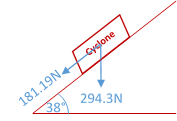
\includegraphics[width=0.4\linewidth]{Images/DT_Fig_16.png}
\caption{Simple force diagram for a wheel on a 38\textordmasculine incline}
\label{fig:simpleforcewheel}
\end{figure}

A force balance using figure \ref{fig:simpleforcewheel} will give the following equation,
\begin{equation}
\sum F_x=F-mgsin\Theta = ma
\end{equation}

Torque ($\tau=F \times r$) can then be substituted into equation D1 and rearranged to get an equation for the torque up an incline.
\begin{equation}
\tau=(a+gsin\Theta)mr
\end{equation}

Given that there are two motors powering Cyclone working at an efficiency below 100\% this should be accounted for and so equation D2 should be divided by the number of motors ($n$) multiplied by their efficiency ($\epsilon$),
\begin{equation}
\tau= \frac{(a+gsin\Theta)mr}{n \epsilon}
\end{equation}

In order to complete this equation the efficiency of the motors and gearhead combination must be estimated. This was done by using the Maxon Motor website and the average efficiencies of likely motors and gearheads that Cyclone would use. The efficiency was estimated to be 60\%, this gives the following result for torque required,
\begin{equation}
\tau= \frac{(0.3+9.81sin38) \times 30 \times 0.05}{2 \times 0.6} = 7.79 Nm
\end{equation}

That is 7.79Nm per motor to accelerate 30kg at 0.3$ms^-2$ up an incline of 38\textordmasculine. The same formula could be used with $a=0 ms^-2$ for Cyclone being held still on the slope, this gives a torque of 7.55Nm (the stall torque).\par

The speed requirement for Cyclone is modified from the previous 2014/15 Orion project, which required a standard operation speed of 1$ms^-1$. This seemed ambitious given the motor and gearhead combinations available and their torque requirement. This prompted the speed requirement to be lowered to $0.5ms^-1$ standard operation, which is more achievable. From this information five motor and gearhead combinations were selected outlined in table \ref{tab:MotorGearSpec}.\par

\begin{table}[h]
\centering
\resizebox{\linewidth}{!}{
\begin{tabular}{p{4cm} s s s s s s s s s}
\hline
Type & Option & \multicolumn{2}{s}{Nominal Speed} & Nominal & Stall & Max Combined  & Gear  & Cost per.  & Length \\
\cline{3-4}
 & & Min V & Max V & Torque & Torque & Efficiency (\%) & Reduction & Combination & \\
\hline
EC 45dia. 15W w/ hall sense w/ GP42C 126:1 gearhead & 1 & 0.21 & 0.25 & 13,1412 & 1540 & 57.6 & 126 & £554.15 & 215.6\\
EC 45dia. 15W w/ hall sense w/ GP42C 126:1 gearhead & 2 &  0.19 & 0.26 & 13,279 & 1600 & 57.6 & 126 & £554.15 & 215.6 \\
RE50 200W 24V GB motor w/ GP52C 26:1 gear & 3 & 0.29 & 0.38 & 8,677.44 & 7370 & 78.02 & 26 & £460.21 & 206.4 \\
EC-4 pole 30dia. 200W 48V w/ GP42C 126:1 gearhead & 4 & 0.17 & 0.22 & 8,292.82 & 3430 & 64.8 & 126 & £505.63 & 155.2 \\
EC-4 pole 30dia. 200W 48V w/ GP32HP 123:1 gearhead & 5 & 0.17 & 0.22 & 7,870.5 & 3430 & 63 & 123 & £526.09 & 155.2 \\
\hline
\multicolumn{10}{c}{Orion's (2014/15) selection} \\
\hline
EC-4 pole 22dia. 200W 48V w/ GP32C 123:1 Gearhead & - & 0.43 & 0.57 & 3,436.84 & 588 & 61.6 & 123 & £718.70 & 122.7 \\
\hline
\end{tabular}
}
\caption{Motor and Gear head specification and selection}
\label{tab:MotorGearSpec}
\end{table}
%$^1$ The options were ranked by 1nominal Torque in descending order.}
%$^2$ The Nominal speed was found by the following equation, ((V×(speed constant)×efficiency)/(gear reduction)). Max V is the maximum voltage that the motor could run at and Min V is the minimum voltage (varies with motors).
%$^3$ The Nominal torque was found using the following equation, (nominal current×torque constant×gear reduction×efficiency).
%$^4$ Stall torque is obtained from the motor specification from Maxon Motor. [RefMotor]
%$^5$ Maximum combined efficiency is found by, (motor efficiency ×gear head efficiency).
%$^6$ Gear Reduction is obtained from the motor specification from Maxon Motor. [RefMotor]
%$^7$ Cost per combination is obtained from the motor specification from Maxon Motor adding cost of motor to cost of gear head. [RefMotor]
%$^8$ Length is obtained from the motor specification from Maxon Motor adding length of motor to length of gear head. [RefMotor]
%RefMotor - http://www.maxonmotor.co.uk/maxon/view/content/index%

As can be seen from table \ref{tab:MotorGearSpec}, the most appropriate motor given the design specifications for Cyclone is the 3rd choice, RE50 200W 24V GB motor with GP52C 26:1 gearhead. This motor does not have as high a torque as option 1 or 2 but does have the highest speed, the greatest stall torque, the best efficiency and is the cheapest option. This option however does not meet the speed requirement of 0.5$ms^-1$. This compromise was accepted on the grounds that the robot must be able to traverse the uneven terrain of a disaster zone and so torque should take priority. As seen in table \ref{tab:MotorGearSpec} the nominal torque (maximum continuous torque) of the chosen combination is 887.44Nm above that of the worst case torque required.\par

%These figure are on the same level%
%Insert figure X17 'Maxon Motor Gearhead, Part no. 370356' (Left aligned)%
\begin{figure}[h]
\centering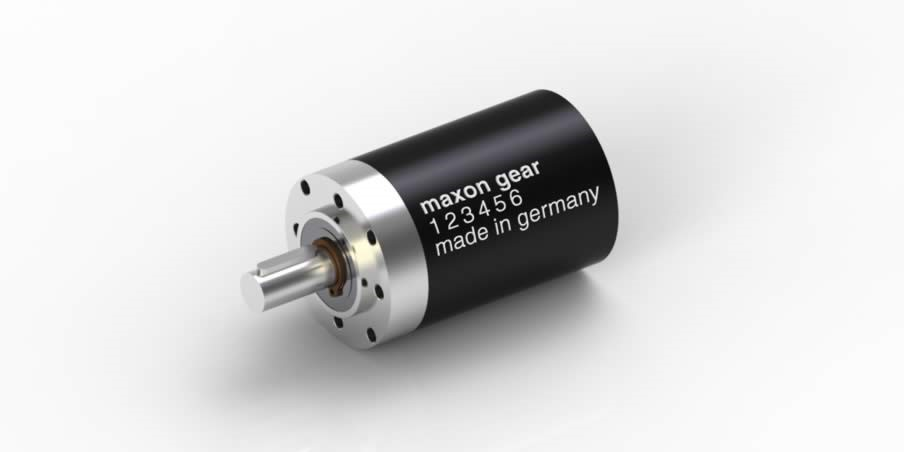
\includegraphics[width=0.6\linewidth]{Images/DT_Fig_17.jpg}
\caption{Maxon Motor Gearhead, Part no. 370356}
\label{fig:gear}
\end{figure}
%Insert figure X18 'Maxon Motor, motor, Part no. 223087' (Right aligned)%
\begin{figure}[h]
\centering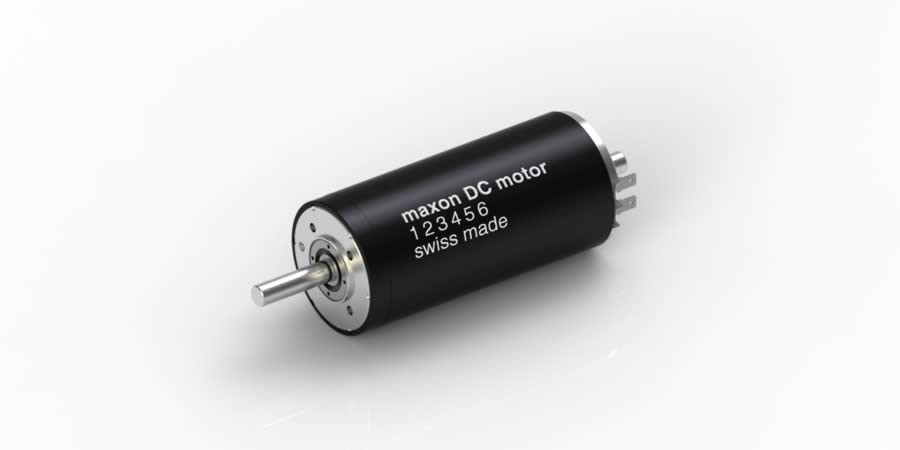
\includegraphics[width=0.6\linewidth]{Images/DT_Fig_18.jpg}
\caption{Maxon Motor, motor, Part no. 223087}
\label{fig:motor}
\end{figure}

The efficiency of this motor and gearhead combination is 78.02\% and therefore the calculation for the torque required to accelerate 30kg at 0.3$ms^-2$ up an incline of 38\textordmasculine can be revised using this new efficiency (equation D5).\par
\begin{equation}
\tau= \frac{(0.3+9.81sin38) \times 30 \times 0.05}{2 \times 0.7802} =6.09 Nm
\end{equation}

That is 6.09Nm per motor for this worst case scenario. The same formula again could be used with $a=0ms^-2$ for Cyclone being held still on the slope, this gives a torque of 5.81Nm (the stall torque). This shows that the motors more than meet the torque requirements of Cyclone.\par

%References- 
%[Ref1] - http://www.intorobotics.com/wheels-vs-continuous-tracks-advantages-disadvantages/
%[Ref2] - https://www.quora.com/Is-there-any-benefit-to-legged-robots-over-wheeled-ones
%[Ref3] - http://www.astro.mech.tohoku.ac.jp/~eric/sitePages/leon.html
%[Refrandom] - http://www.simbotics.org/files/pdf/drivetraindesign.pdf
%[Refrandom] - https://en.wikipedia.org/wiki/Steering
%[RefSkidsteer] - http://groups.csail.mit.edu/drl/courses/cs54-2001s/skidsteer.html
%[RefAlternativeDrivetrain] - http://www.altfuels.org/backgrnd/altdrive.shtml
%[RefSteering] - http://www.gizmology.net/tracked.htm
%[RefMotor] - http://www.maxonmotor.co.uk/maxon/view/content/index
